\chapter{Signal Modeling}

How do we produce a signal hypothesis that we can test?
Mostly just a bunch of software.

\section{Monte-Carlo Simulation} \label{sec:mcsim}

    The process of simulating physics events is done in many steps, using a suit of different software programs.

    The signal simulation samples used in this analysis proceed through a production chain of three programs
        -- MadGraph, Pythia8, and Geant4 -- before going through the reconstruction and selection processes described in Chapters \ref{ch:reconstruction} and \ref{ch:selection}.

    MadGraph is used to simulate the feynman-diagram process of VBF \to HH \to 4b.
    It generates a bunch of events with output kinematics.

    Pythia8 is used to simulate particle decay, showering, and radiation.

    Geant4 simulates the entirety of the ATLAS detector.
    The particles and showers output by Pythia8 are propogated through the materials of the ATLAS machine by Geant4,
        with further showering and scattering effects modeled.
    The detectors' response to the simulated particles are recorded, with the detector output stored in the same format as that produced by the ATLAS hardware.

\section{Signal Combination}

    As discussed in Section \ref{sec:feyn_rules}, the cross-section and kinematic distributions of the di-Higgs production processes depend fundamentally on a number of coupling constants between the Higgs and other particles.
    Of particular interest in this analysis are \kl for the Higg's self-coupling and \kvv for the \HHVV coupling.
    The values of \kl and \kvv have loose experimental constraints \cite{EXOT-2016-31} \cite{HDBS-2018-18-witherratum} \cite{ATLAS-CONF-2019-049},
        requiring analysis across a wide range of these coupling values.
    Unfortunately, MC generation is computationally expensive and time consuming.
    As such, only a handful of MC simulation samples for only a handful of coupling values are actually produced,
        and a sample combination technique is employed to model the signal hypothesis across the coupling parameter space.

    The process of combining a few samples in such a way as to model the entire parameter space of coupling constants is based on exploiting the underlying mathematics of the differential cross-section formula.
    By expanding the squared term of the sum of all Feynman diagram contributions,
        the cross-section can be expressed as a function of its coupling values \cite{ATLAS-CONF-2019-049}, as shown in Equation \ref{eq:tree_level_invamp}.
    Rewritting the expression again in terms of the cross-section as a function of the observable \mhh:

    \begin{equation} \begin{split} \label{eq:tree_level_invamp_simple}
        \dXsecM &\propto |\invAmp|^2 = |  \kv^2 M_t + \kv \kl M_s + \kvv M_x |^2 \\
        &\propto \kv^2 \kl^2 a_1 + \kv^4 a_2 + \kvv^2 a_3 + \kv^3 \kl a_4 + \kv \kl \kvv a_5 + \kv^2 \kvv a_6
    \end{split} \end{equation}

    The $a_i$ matrix element expansion values have a dependence on \mhh, which is not trivially derivable as an analytic function.
    Instead, for a given coupling, its cross-section for a given \mhh can be mathematically determined by solving a set of linear equations for the $a_i$ terms.
    This is done using six different cross-section values (for the same \mhh) for six different coupling values.
    In practice, the cross-section values of these six \textit{basis} samples are represented by their yields from MC simulation, binned by their \mhh.
    These six samples (rather, their \mhh-binned MC yields) are then combined using the aformentioned linear equations.
    Due to the complexities of the kinematics of the VBF process,
        the samples used in the combination must have already been run through the full reconstruction and selection process detailed in Section \ref{sec:mcsim}.
    The signal distribution modelling is thus performed by directly combining the reconstructed \mhh distributions of post-selection signal samples.

    In theory, with infinite events, the only requirement for these samples is that they are linearly independent of each other.
    In practice, the final samples are statistically limited, and different combinations of variations yield different statistical power.
    The 6-sample combination used in this analysis (\ref{tab:vbf_hh_6term_varlist} and \ref{eqn:vbf_hh_6term_chosen}) has been chosen specifically for its ability to avoid mismodelling errors.

    \begin{table}[] \centering
    \caption{6-Term VBF Combination Sample Variations}
    \label{tab:vbf_hh_6term_varlist}
    \begin{tabular}{ |l|l|l| }
        \hline
        \textbf {$\kappa_{2V}$} & \textbf {$\kappa_\lambda$} & \textbf {$\kappa_V$} \\
        \hline
            1   &   1 & 1   \\
            1.5 &   1 & 1   \\
            1   &   2 & 1   \\
            1   &  10 & 1   \\
            1   &   1 & 0.5 \\
            0   &  -5 & 0.5 \\
        \hline
    \end{tabular} \end{table}

    \begin{equation}
    \label{eqn:vbf_hh_6term_chosen}
    \begin{split}
        \frac{d\sigma}{d\mhh}(\kvv, \kl, \kv) =
            \left(\frac{68 \kappa_{2V}^{2}}{135} - 4 \kappa_{2V} \kappa_{V}^{2} + \frac{20 \kappa_{2V} \kappa_{V} \kappa_{\lambda}}{27} + \frac{772 \kappa_{V}^{4}}{135} - \frac{56 \kappa_{V}^{3} \kappa_{\lambda}}{27} + \frac{\kappa_{V}^{2} \kappa_{\lambda}^{2}}{9}\right) \times \frac{d\sigma}{d\mhh}{\left(1,1,1 \right)} \\
            + \left(- \frac{4 \kappa_{2V}^{2}}{5} + 4 \kappa_{2V} \kappa_{V}^{2} - \frac{16 \kappa_{V}^{4}}{5}\right) \times \frac{d\sigma}{d\mhh}{\left(\frac{3}{2},1,1 \right)} \\
            + \left(\frac{11 \kappa_{2V}^{2}}{60} + \frac{\kappa_{2V} \kappa_{V}^{2}}{3} - \frac{19 \kappa_{2V} \kappa_{V} \kappa_{\lambda}}{24} - \frac{53 \kappa_{V}^{4}}{30} + \frac{13 \kappa_{V}^{3} \kappa_{\lambda}}{6} - \frac{\kappa_{V}^{2} \kappa_{\lambda}^{2}}{8}\right) \times \frac{d\sigma}{d\mhh}{\left(1,2,1 \right)} \\
            + \left(- \frac{11 \kappa_{2V}^{2}}{540} + \frac{11 \kappa_{2V} \kappa_{V} \kappa_{\lambda}}{216} + \frac{13 \kappa_{V}^{4}}{270} - \frac{5 \kappa_{V}^{3} \kappa_{\lambda}}{54} + \frac{\kappa_{V}^{2} \kappa_{\lambda}^{2}}{72}\right) \times \frac{d\sigma}{d\mhh}{\left(1,10,1 \right)}  \\
            + \left(\frac{88 \kappa_{2V}^{2}}{45} - \frac{16 \kappa_{2V} \kappa_{V}^{2}}{3} + \frac{4 \kappa_{2V} \kappa_{V} \kappa_{\lambda}}{9} + \frac{152 \kappa_{V}^{4}}{45} - \frac{4 \kappa_{V}^{3} \kappa_{\lambda}}{9}\right) \times \frac{d\sigma}{d\mhh}{\left(1,1,\frac{1}{2} \right)} \\
            + \left(\frac{8 \kappa_{2V}^{2}}{45} - \frac{4 \kappa_{2V} \kappa_{V} \kappa_{\lambda}}{9} - \frac{8 \kappa_{V}^{4}}{45} + \frac{4 \kappa_{V}^{3} \kappa_{\lambda}}{9}\right) \times \frac{d\sigma}{d\mhh}{\left(1,-5,\frac{1}{2} \right)}
    \end{split}
    \end{equation}

    The method used to determine the overall performance of a basis is to check the number of negative bins generated
        in the \mhh distribution across all points in the two-dimensional \kvv,\kl space, as seen in \ref{fig:vbf_hh_6term_nWeight_grid}.
    As negative bin weights are unphysical, they indicate poor signal modelling.
    Thus, identifying a basis which minimizes the presence of negative weights ensures stable modeling of the signal hypothesis at all points in the coupling space (\ref{fig:vbf_hh_6term_validation} and \ref{fig:vbf_hh_6term_preview}).

    \begin{figure}
        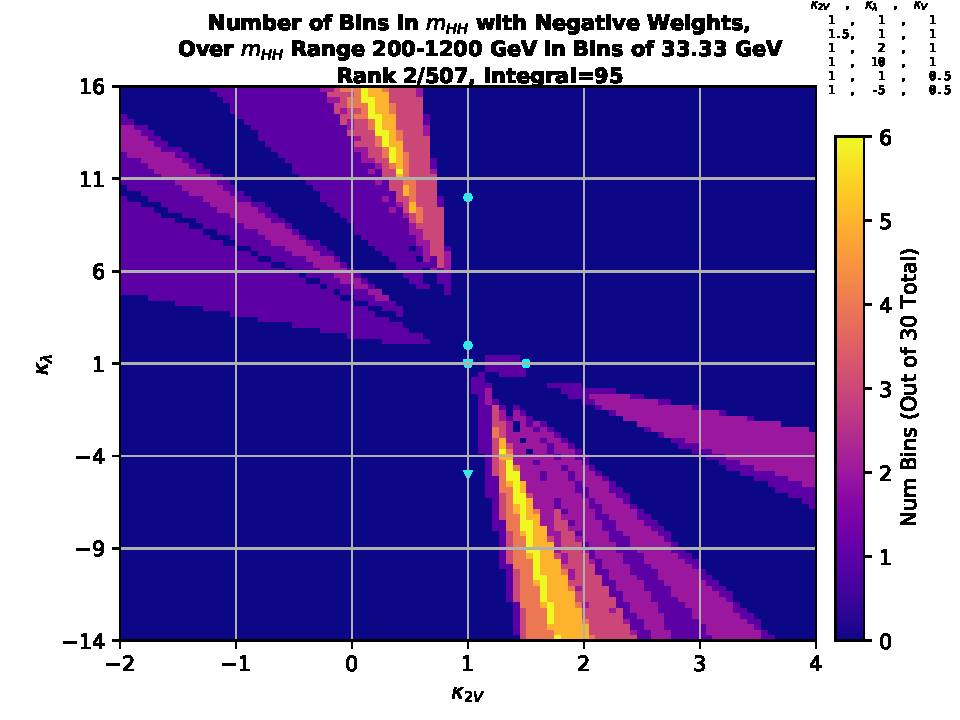
\includegraphics[width=\linewidth,height=\textheight,keepaspectratio]{signal/negative_weights_base}
        \caption{
            Frequency of negative bin weights in \mhh distribution across \kvv,\kl range.
            Brighter regions indicate more negative-weighted bins, and suggest less stable signal modelling.
            This particular combination of samples was chosen for how much of the space is ``dark",
                with darker regions indicating generally stable signal modelling.
            The table of coupling values in the upper right corner indicates the 6 MC samples
                (highlighted on the plot with cyan dots) used in the combination.
        }
        \label{fig:vbf_hh_6term_nWeight_grid}
    \end{figure}

    Ultimately however, the final arbiter of a well constructed basis is that it produces observable distributions comparable to what would be produced through direct MC generation.
    A number of validation tests are thus performed, comparing the distributions from the combination to an already existing MC sample.
    Displayed in Figure \ref{fig:vbf_hh_6term_validation}, the combination shows strong agreement with the MC sample.

    \begin{figure}
        \subfloat[Validation \kv = 1.5]{
            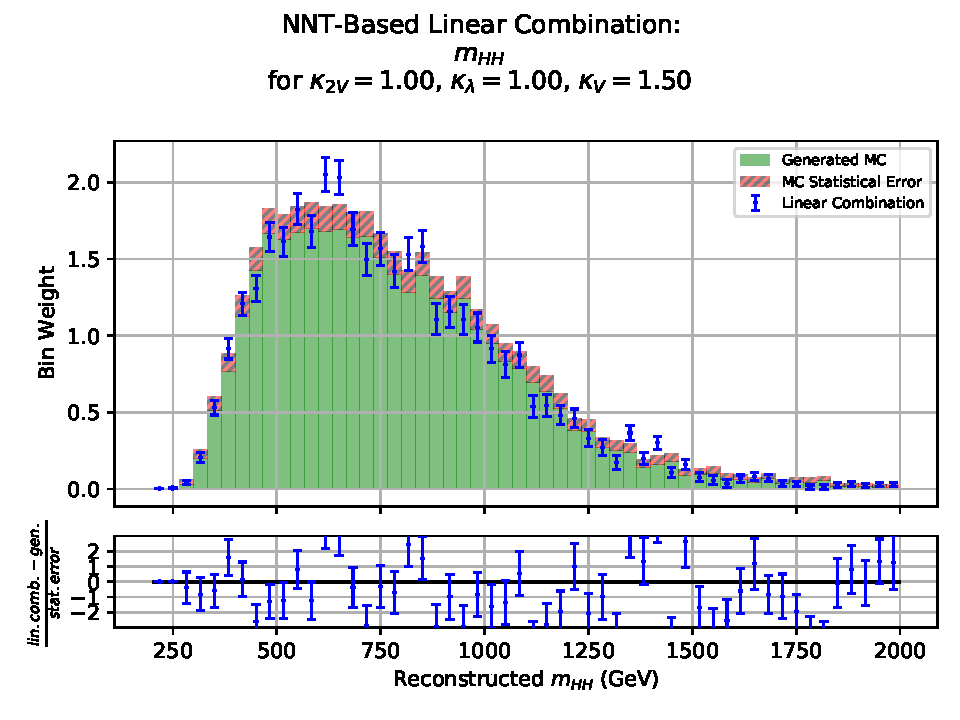
\includegraphics[width=0.5\linewidth,height=\textheight,keepaspectratio]{signal/reco_mHH_cvv1p00cl1p00cv1p50}
        }
        \subfloat[Validation \kl = 0]{
            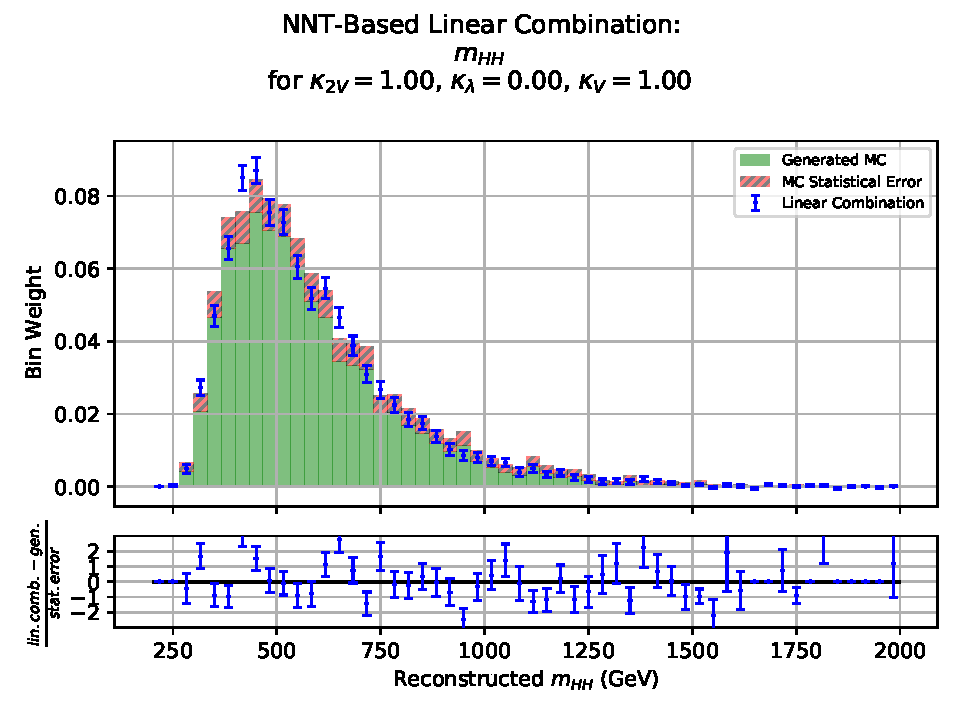
\includegraphics[width=0.5\linewidth,height=\textheight,keepaspectratio]{signal/reco_mHH_cvv1p00cl0p00cv1p00}
        }
        \caption{
            Validation of 6-term combination against MC generated at \kv = 1.5 and \kl = 0.
            The combination shows good agreement to the generated MC distributions.
        }
        \label{fig:vbf_hh_6term_validation}
    \end{figure}

    \begin{figure}
    	\centering
        \subfloat[Validation against MC with $\kl=0$]{
            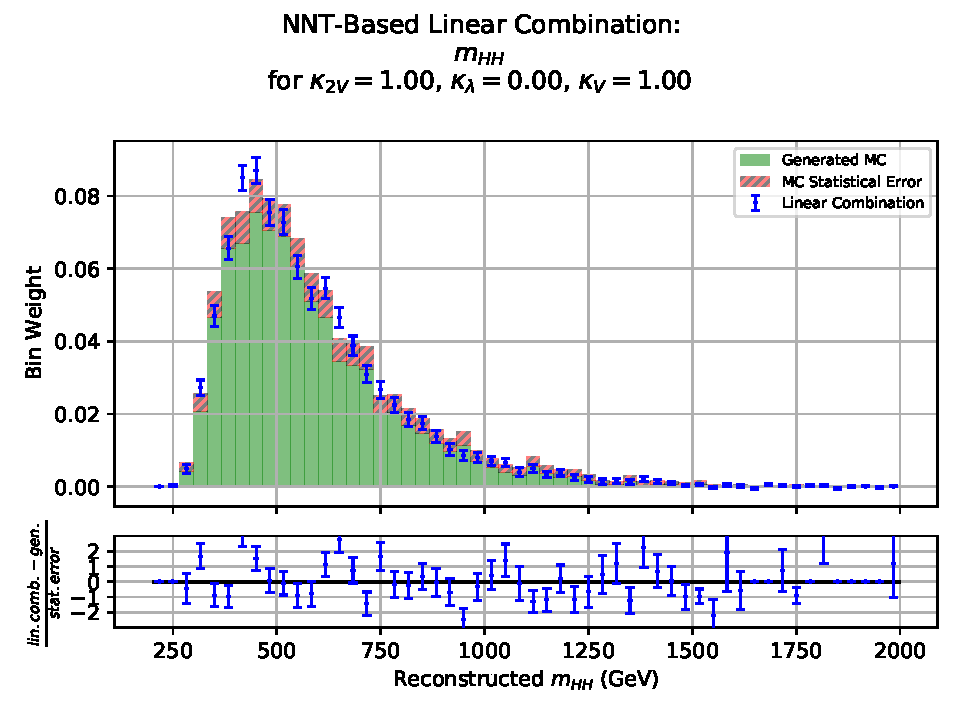
\includegraphics[width=0.32\linewidth,height=\textheight,keepaspectratio]{signal/reco_mHH_cvv1p00cl0p00cv1p00}
        }
        \subfloat[Validation against MC with $\kvv=0$]{
            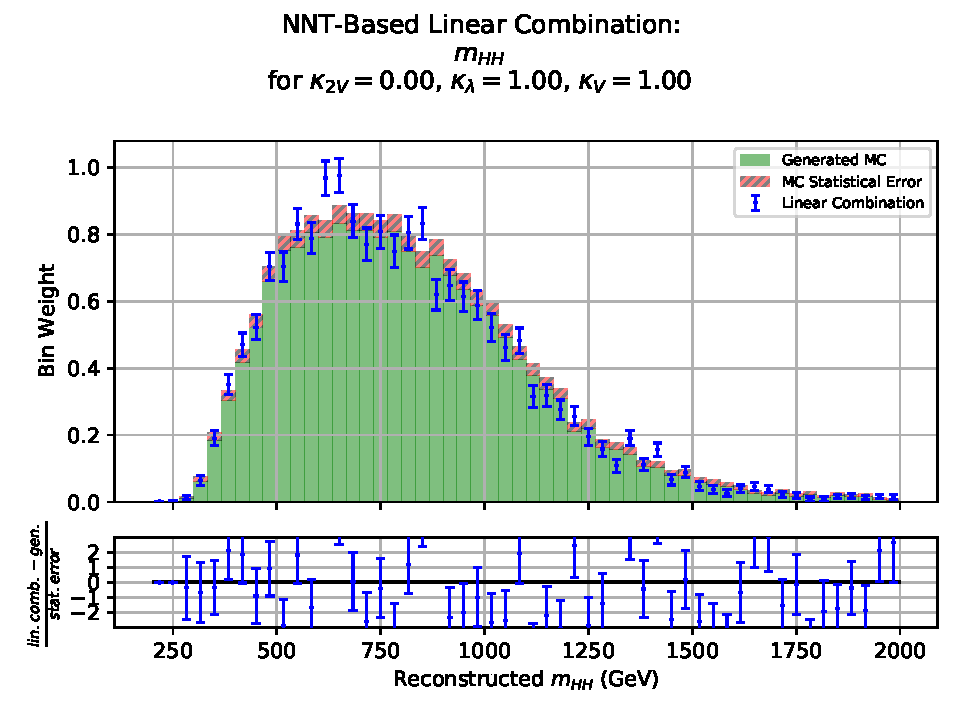
\includegraphics[width=0.32\linewidth,height=\textheight,keepaspectratio]{signal/reco_mHH_cvv0p00cl1p00cv1p00}
        }
        \subfloat[Validation against MC with $\kvv=3$]{
            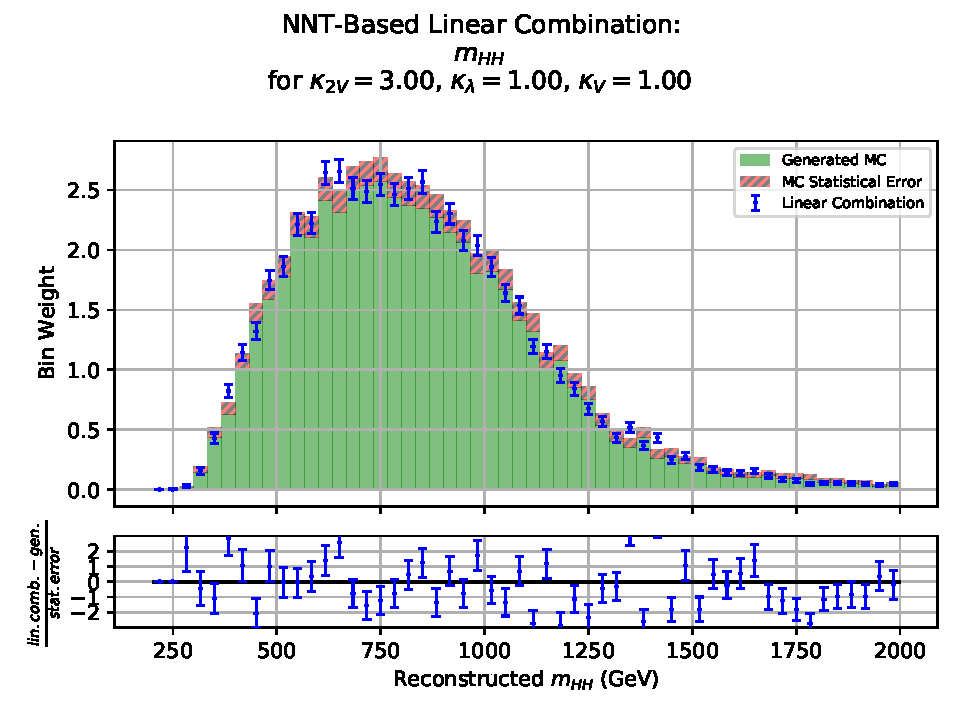
\includegraphics[width=0.32\linewidth,height=\textheight,keepaspectratio]{signal/reco_mHH_cvv3p00cl1p00cv1p00}
        }
        \caption{
            The six-term linear combination of samples is combined for various coupling values.
            The combined distribution shape (in blue) is compared against a Monte-Carlo sample (in green) which was generated for the same coupling values.
            The combination approach shows good agreement with the generated sample, indicating accurate modelling of the signal shape.
        }
        \label{fig:vbf_hh_validation}
    \end{figure}

    As an additional test, I also checked the distribution shape predicted by the combination at points far from the SM.
    These points have no MC samples to compare to, but the points can still be checked to ensure they at least look well-behaved.

    \begin{figure}
        \subfloat[Combined \mhh distribution at \kvv = 2.5, \kl = -10]{
            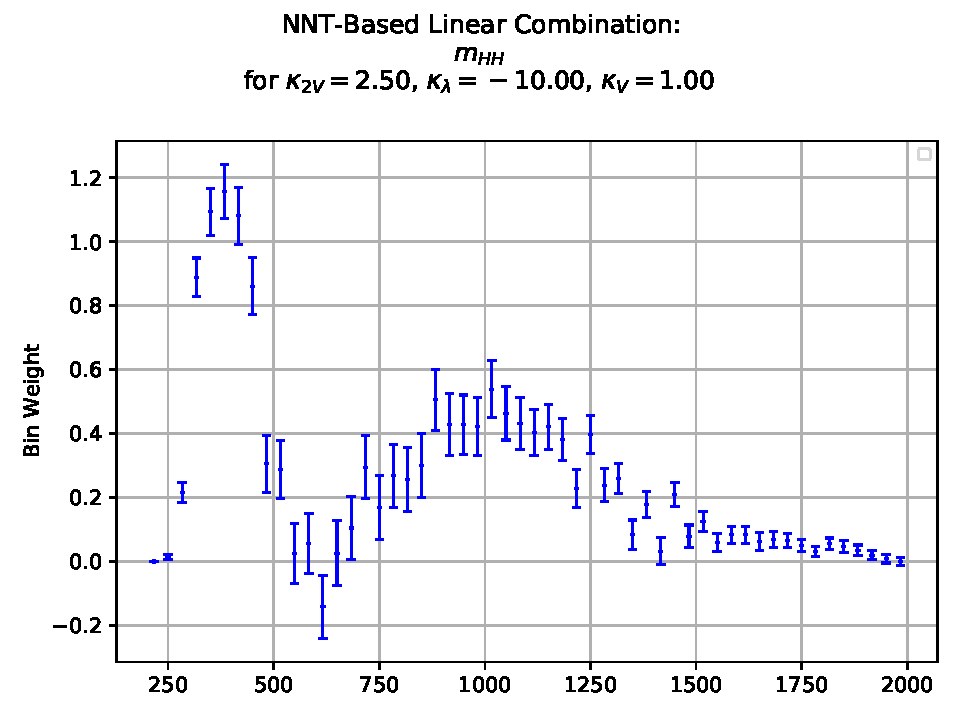
\includegraphics[width=0.5\linewidth,height=\textheight,keepaspectratio]{signal/preview_reco_mHH_new_cvv2p50cl-10p00cv1p00}
        }
        \subfloat[Combined \mhh distribution at \kvv = 2.0, \kl = -10]{
            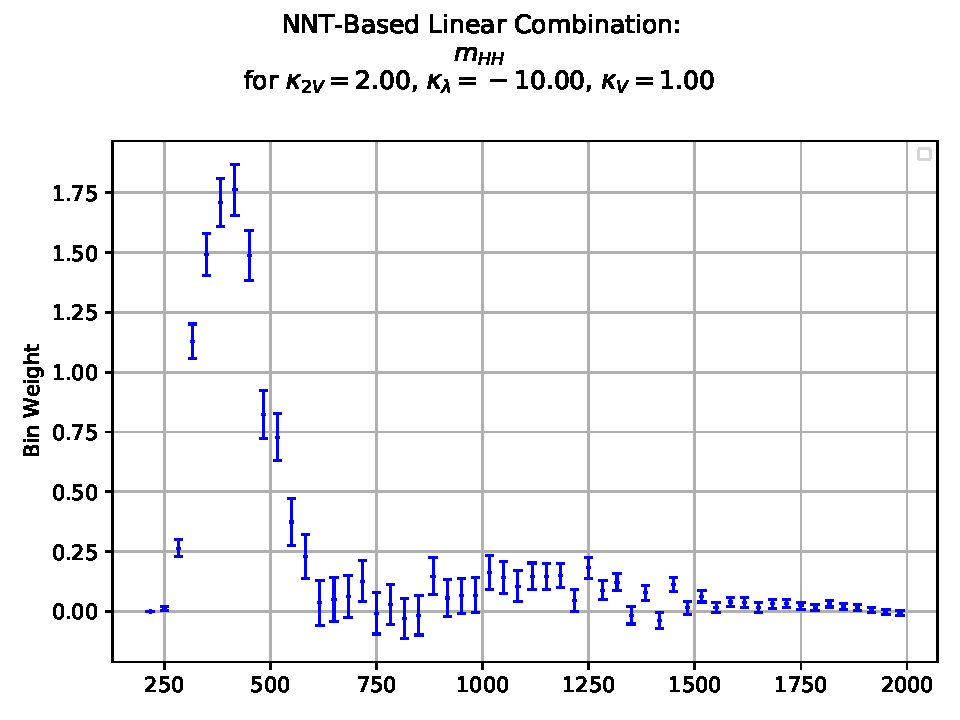
\includegraphics[width=0.5\linewidth,height=\textheight,keepaspectratio]{signal/preview_reco_mHH_new_cvv2p00cl-10p00cv1p00}
        }\\
        \subfloat[Combined \mhh distribution at \kvv = 0, \kl = 13]{
            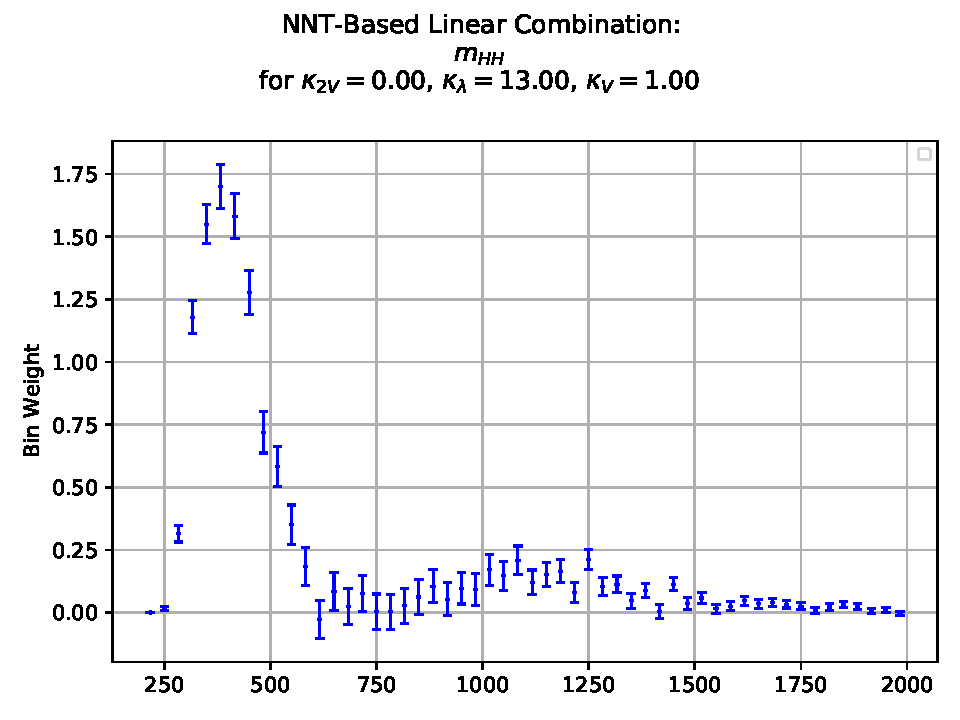
\includegraphics[width=0.5\linewidth,height=\textheight,keepaspectratio]{signal/preview_reco_mHH_new_cvv0p00cl13p00cv1p00}
        }
        \caption{
            \mhh distribution produced by the 6-term combination at points far from the SM.
            The combination produces smooth, well-behaved distributions at these points,
                suggesting the signal is well-modelled in these regions.
        }
        \label{fig:vbf_hh_6term_preview}
    \end{figure}

    \begin{figure}
    	\centering
        \subfloat[Combination at  \kvv = -2]{
            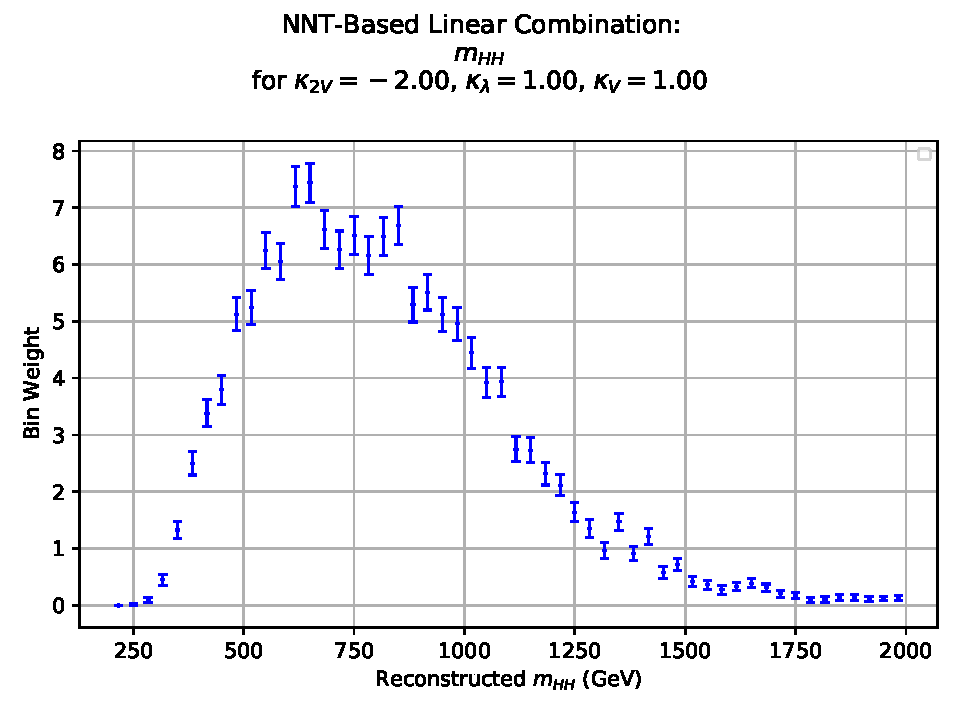
\includegraphics[width=0.44\linewidth,height=\textheight,keepaspectratio]{signal/preview_reco_mHH_new_cvv-2p00cl1p00cv1p00}
        }
        \subfloat[Combination at  \kl = -9]{
            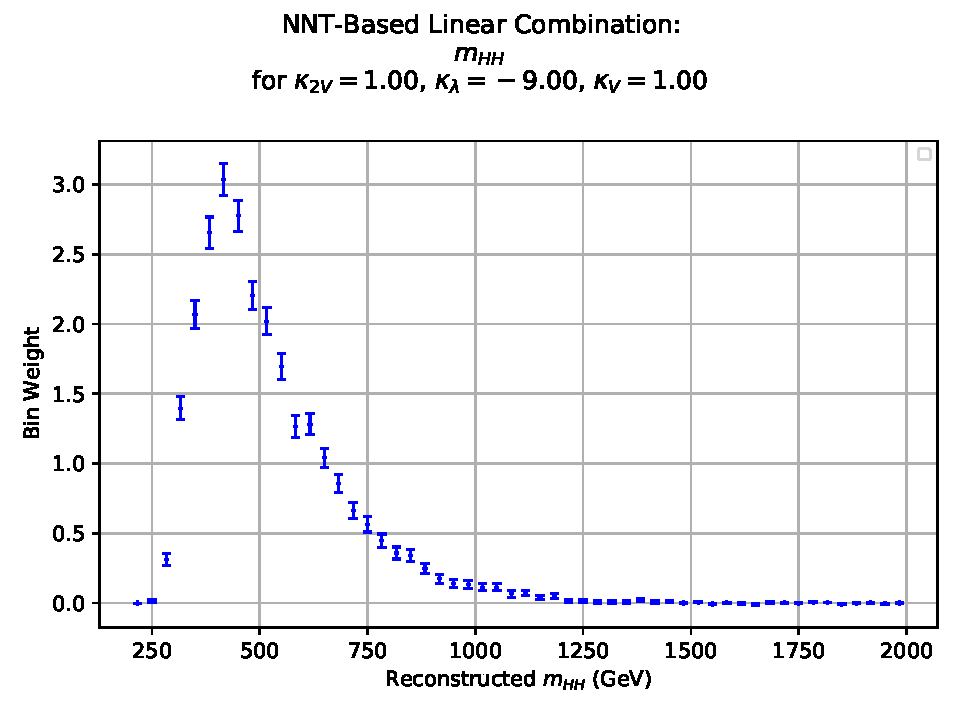
\includegraphics[width=0.44\linewidth,height=\textheight,keepaspectratio]{signal/preview_reco_mHH_new_cvv1p00cl-9p00cv1p00}
        }
        \caption{
            The six-term linear combination of samples is combined for coupling values very far from the Standard Model.
            There are no MC simulated samples to compare these points too, but the combined distributions at these points are smooth and well-behaved,
                indicating reasonable modelling of the distribution even at distant couplings.
        }
        \label{fig:vbf_hh_preview}
    \end{figure}


\section{Solidarity}
    
    Should this go here?
